\documentclass{beamer}
\usepackage{minted}
\usepackage{hyperref}
\usepackage[style=numeric]{biblatex}
\usepackage{subfig}
%\addbibresource{main.bib}
\usepackage{xcolor}
\usetheme{metropolis}

\definecolor{cvutblue}{RGB}{1,44,86}

\newcommand{\reffig}[1]{Fig.~\ref{#1}}
\newcommand{\reflst}[1]{Lst.~\ref{#1}}
\newcommand{\refalg}[1]{Alg.~\ref{#1}}
\newcommand{\refsec}[1]{Sec.~\ref{#1}}
\newcommand{\reftab}[1]{Table~\ref{#1}}
\newcommand{\refeq}[1]{\eqref{#1}}

\newcommand{\todo}[1]{{\color{red} TODO {#1}}}

\setbeamercolor{palette primary}{bg=cvutblue,fg=white}
\setbeamercolor{background canvas}{bg=white}

\setbeamertemplate{footline}[frame number]

\newcounter{questionnumber}
\newcommand{\questionframe}[2]{
    \stepcounter{questionnumber}
    {
    \setbeamertemplate{footline}{}
    \begin{frame}{Question \arabic{questionnumber}}
        \addtocounter{framenumber}{-1}
        \begin{block}{#1}
        \vspace{0.5cm}
            #2
        \end{block}
    \setbeamertemplate{footline}[frame number]
    \end{frame}
    }
}


\title{Relative Pose Estimation Using Event-Based Measurements of LED Signals}

\date{31.4.2222}
\author{Jakub Pelc}

\institute{Faculty of Electrical Engineering, Czech Technical University in Prague}
\begin{document}
\maketitle

\begin{frame}{Assignment}

\small{
\begin{enumerate}
    \item Research the working principles of event-based cameras. Research the existing Visible Light Positioning (VLP) methods such as Received Signal Strength Ratio (RSSR).
    \item Analyze the response of a static event-based camera to UV LEDs used by the UVDAR localization system in UAV swarms. Modulate the signals with varying frequency, relative distance, and angle.
    \item Design an approach for relative pose estimation of UAV swarm members, utilizing the analysis results and a proper
fisheye lens calibration method.
    \item Implement the proposed solution for a Robot Operating System (ROS). Test the implementation on the data used for
the response analysis and discuss the results.
    \item Conduct a real-world UAV swarming experiment. Compare the estimation results with a GNSS ground truth. 
\end{enumerate}
}

\end{frame}

\begin{frame}{Event-based cameras}
The event-based cameras capture the logarithmic brightness changes on each camera pixel, if a certain threshold is crossed, an event is generated.

\begin{figure}[H]
    \centering
    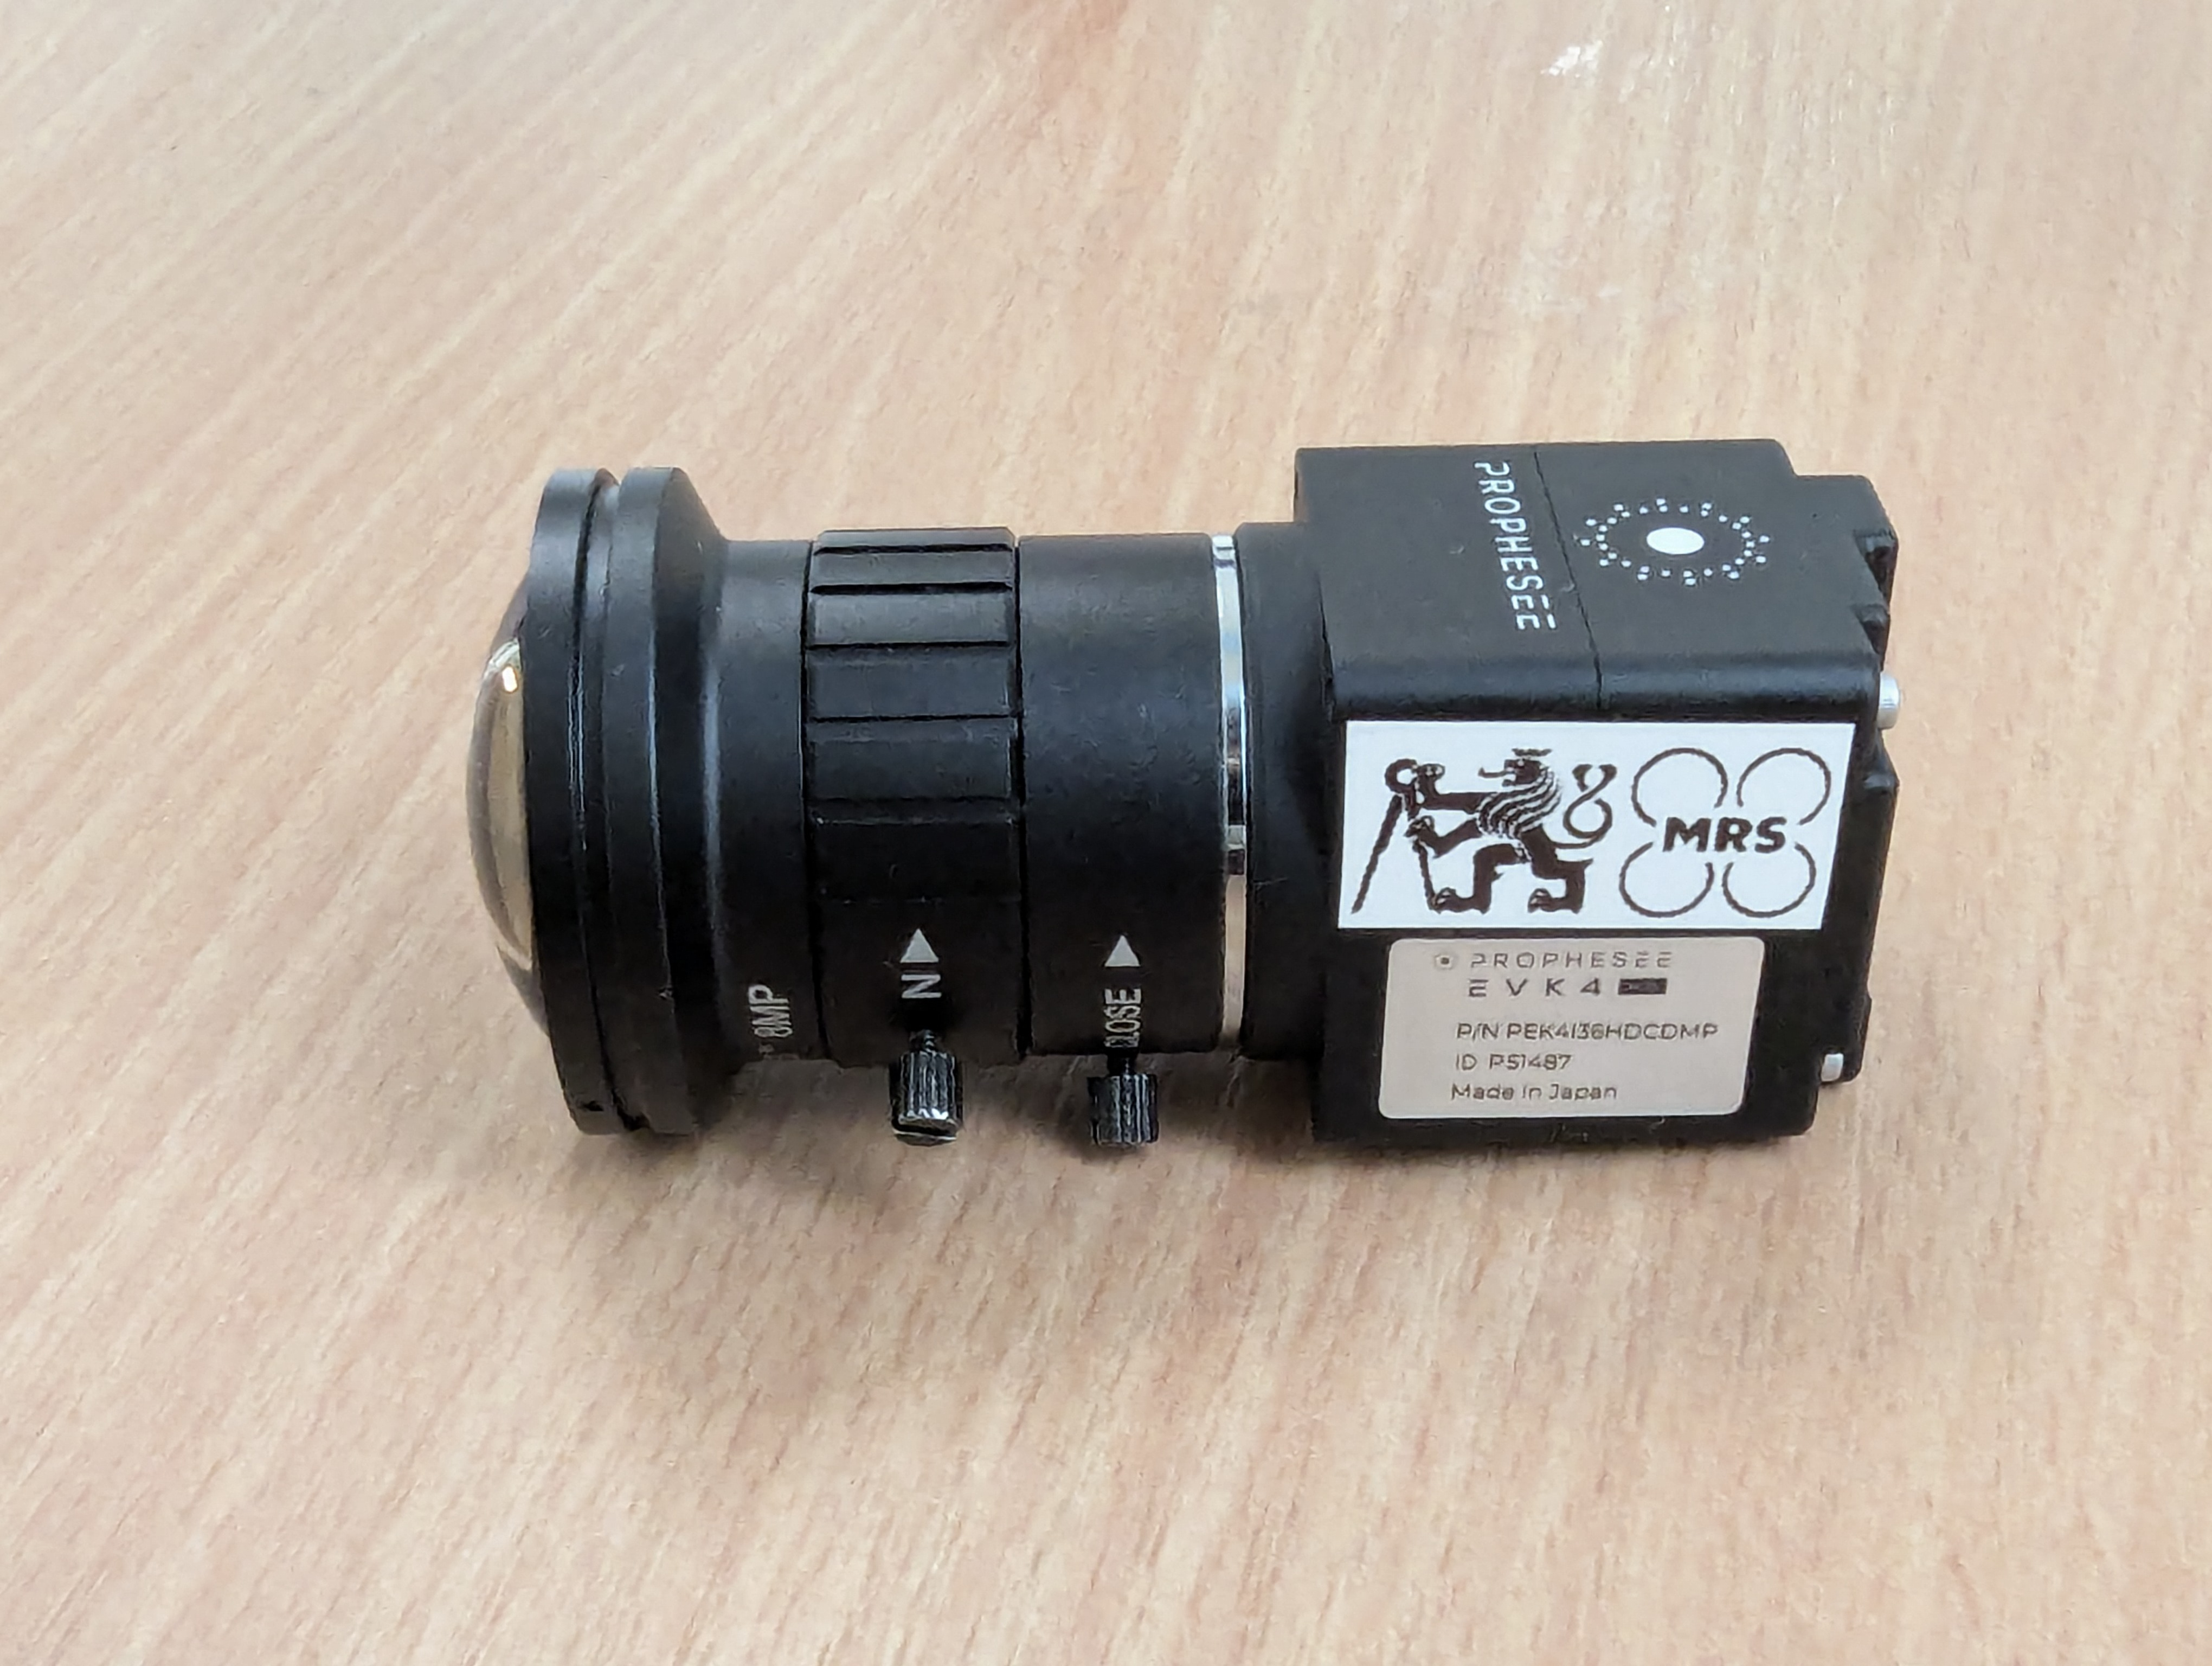
\includegraphics[width=0.374\textwidth]{../fig/photos/evk4.jpg}
    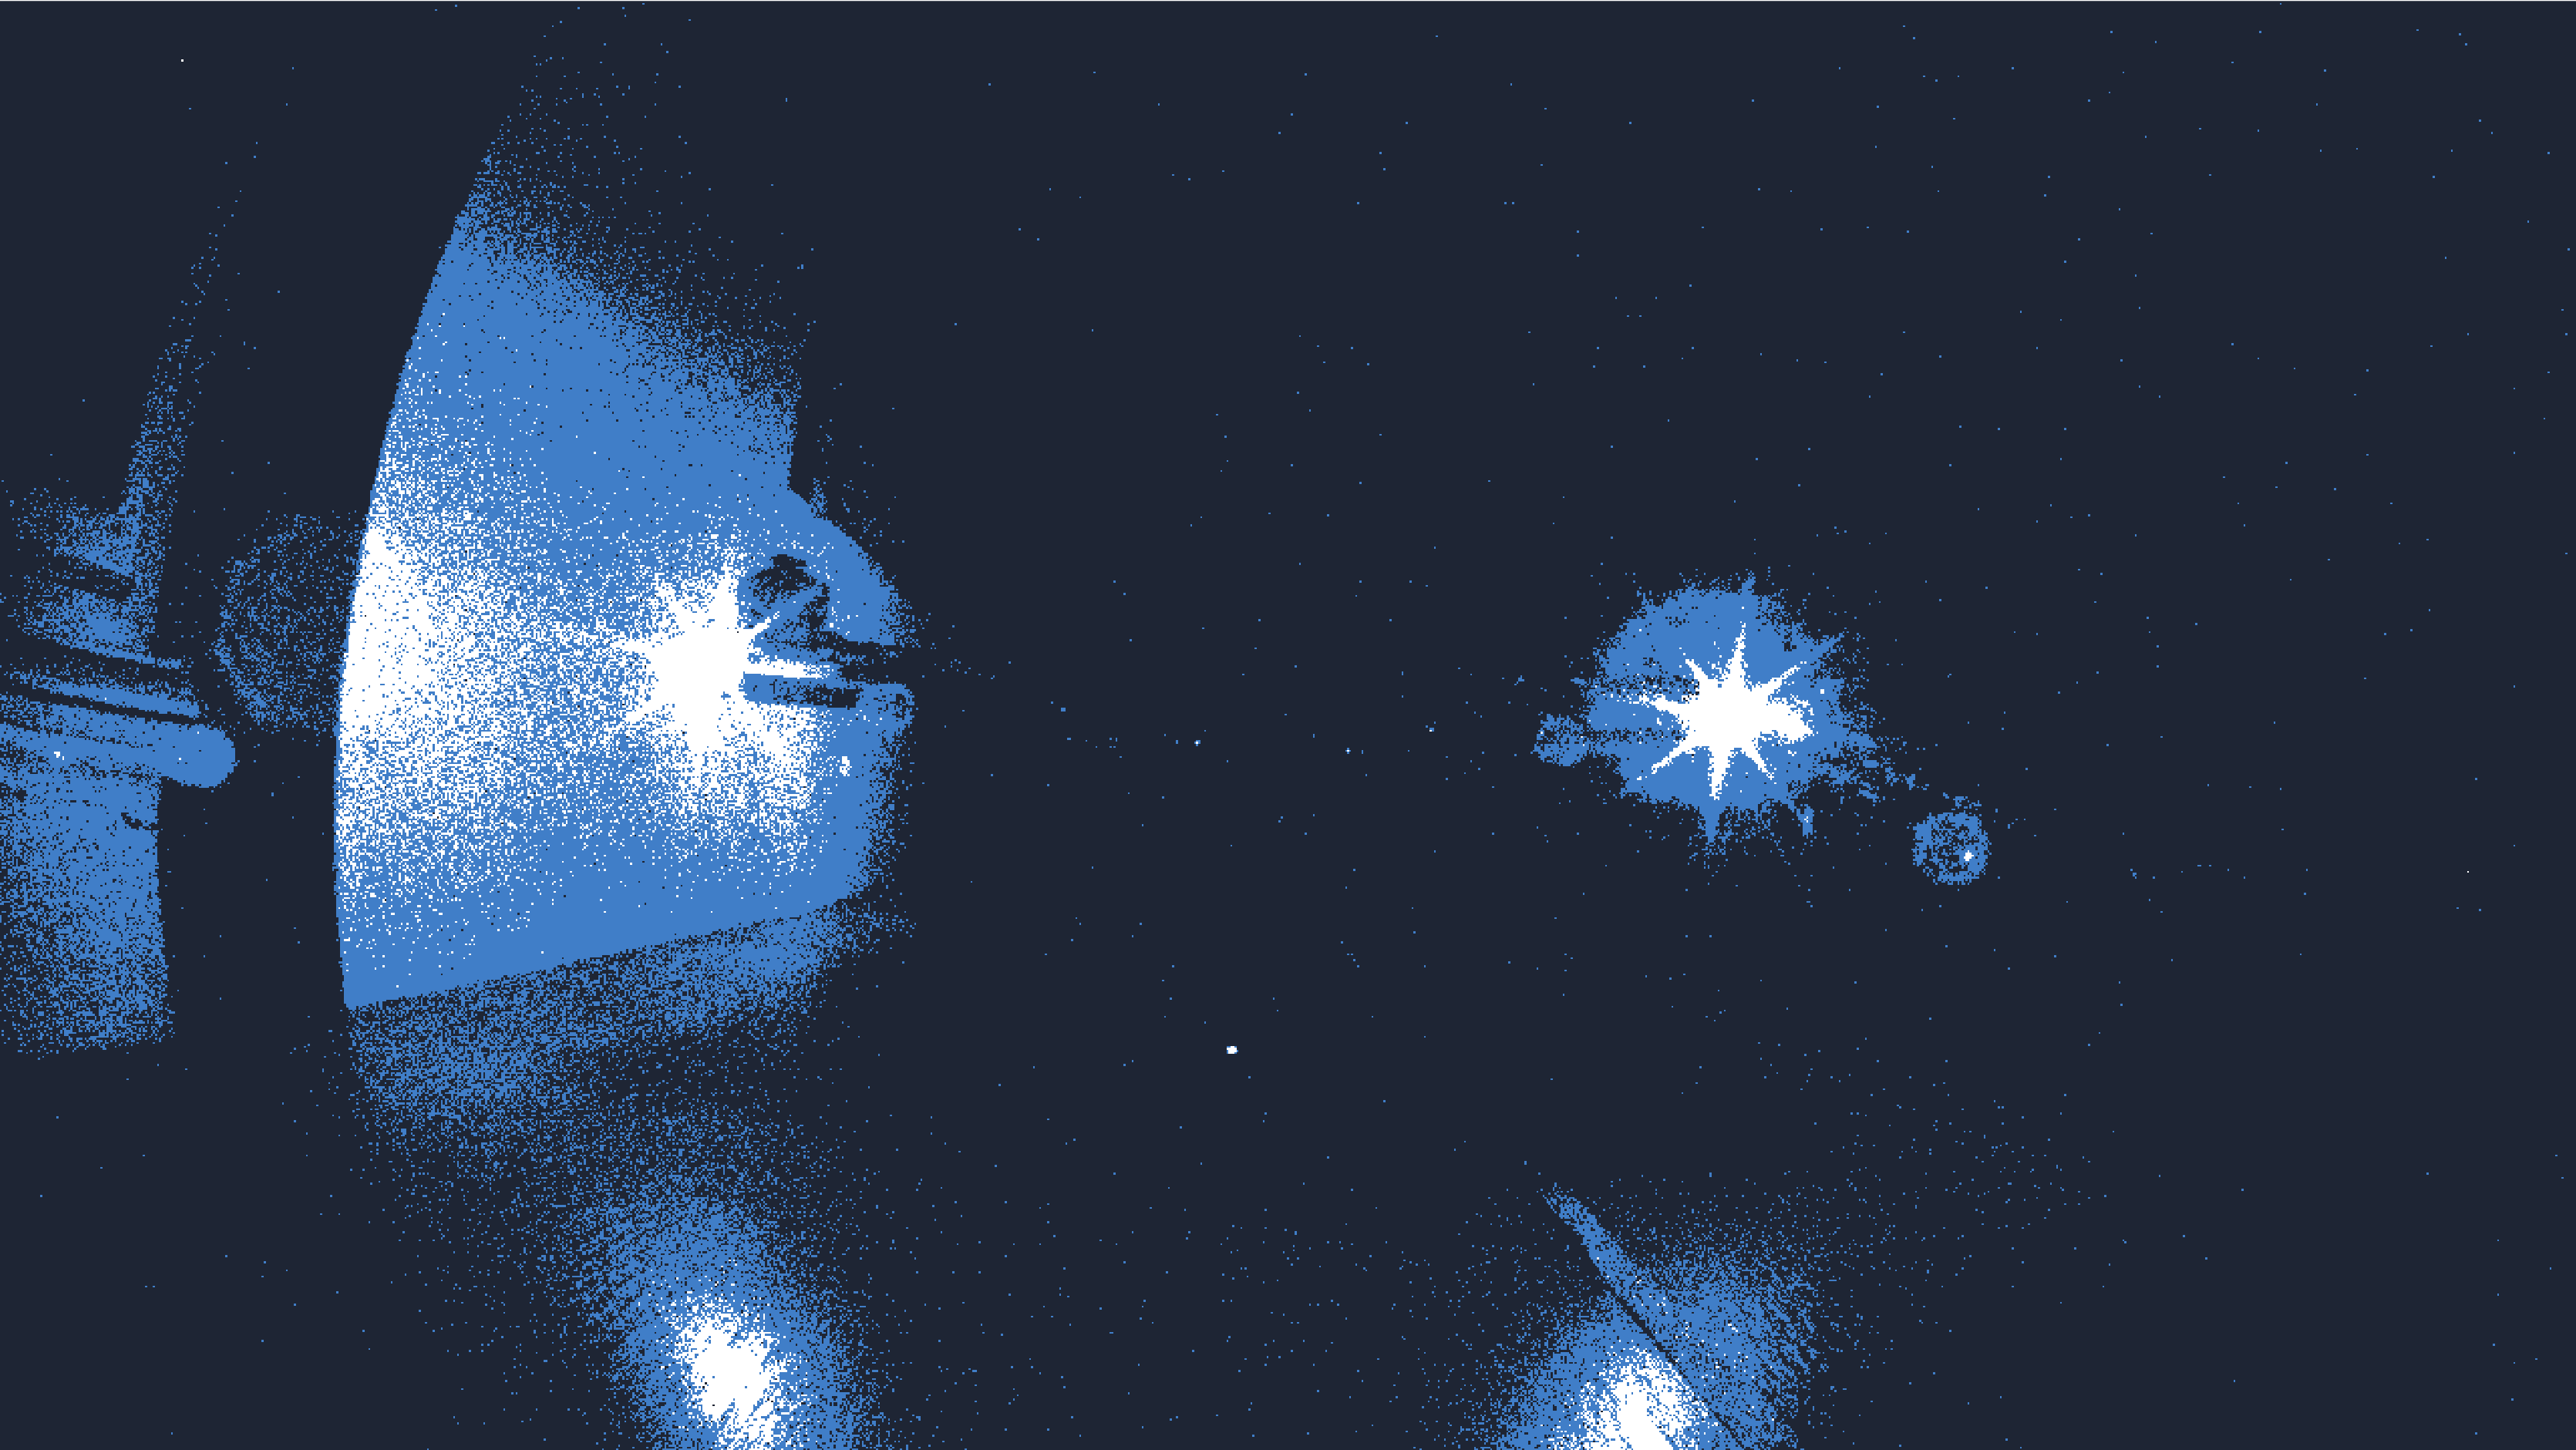
\includegraphics[width=0.50\textwidth]{../fig/photos/meas1.png}
    \label{fig:evk4}
\end{figure}

We observe a UAV equipped with the UVDAR system, which controls the UV LEDs, and allows for their modulation.

\end{frame}

\begin{frame}{Distance influence}

\begin{figure}[H]
    \centering
    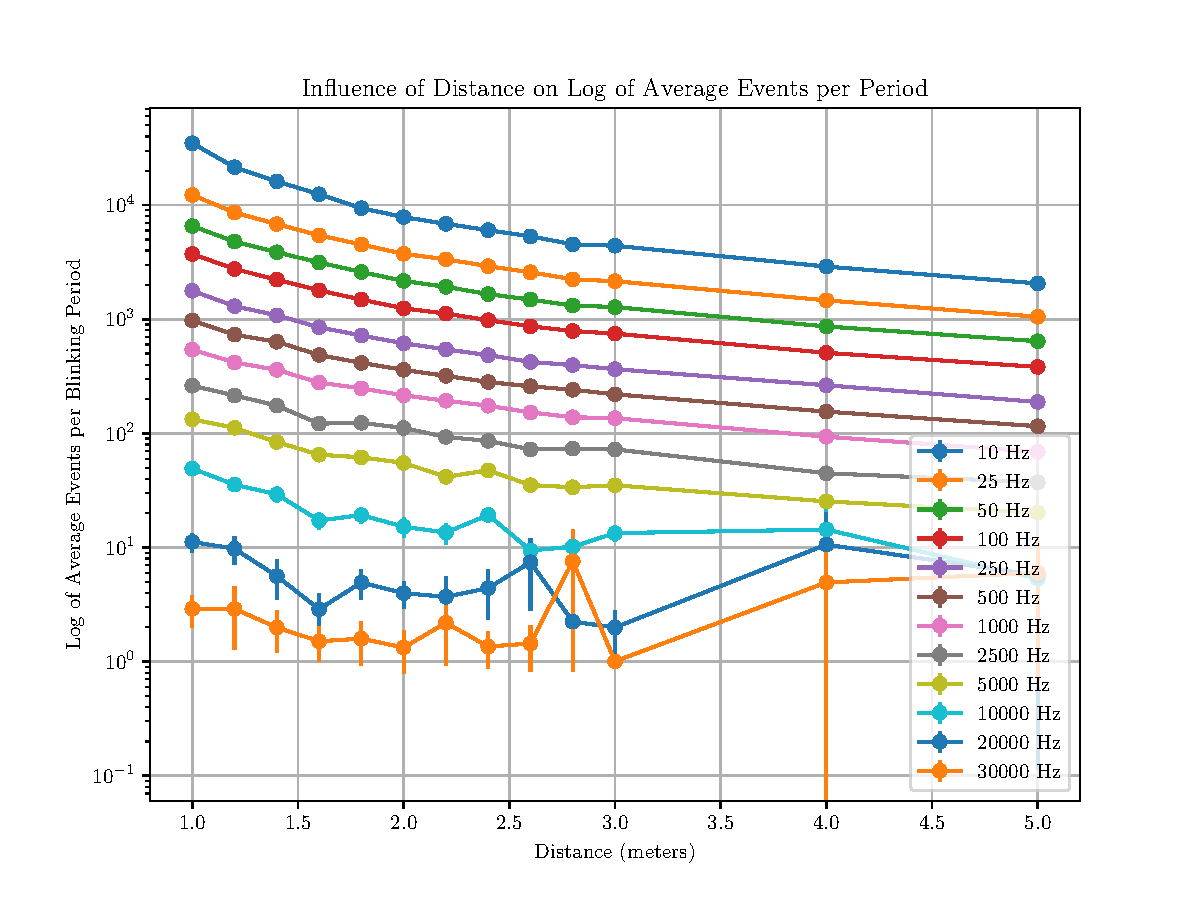
\includegraphics[width=0.8\textwidth]{../fig/semestral/distlog.pdf}
    \label{fig:dist_influence}
    \caption{Distance influence}
\end{figure}

\end{frame}

\begin{frame}{Frequency influence}

\begin{figure}[H]
    \centering
    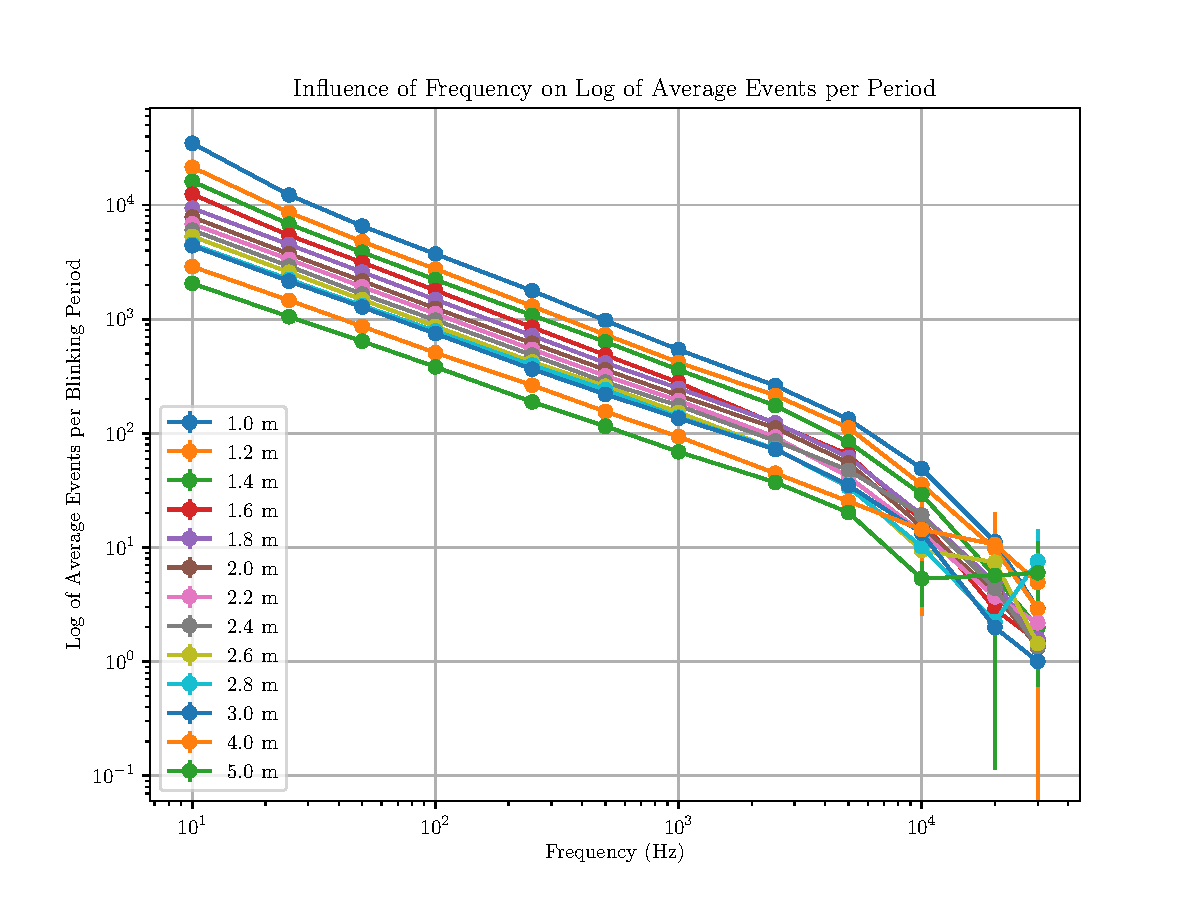
\includegraphics[width=0.8\textwidth]{../fig/semestral/freqlog.pdf}
    \label{fig:freq_influence}
    \caption{Frequency influence}
\end{figure}

\end{frame}

\begin{frame}{Rotation influence}

\begin{figure}[H]
    \centering
    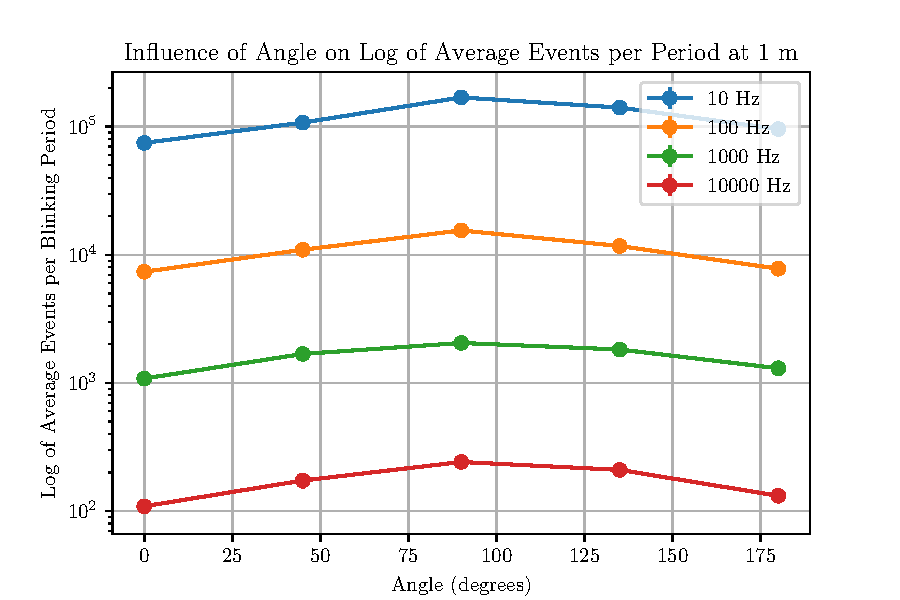
\includegraphics[width=0.8\textwidth]{../fig/semestral/angle2.pdf}
    \label{fig:rotation_influence}
    \caption{Rotation angle influence}
\end{figure}

\end{frame}

\begin{frame}{Experimental validation of the inverse square law}

    \begin{figure}
        \centering
        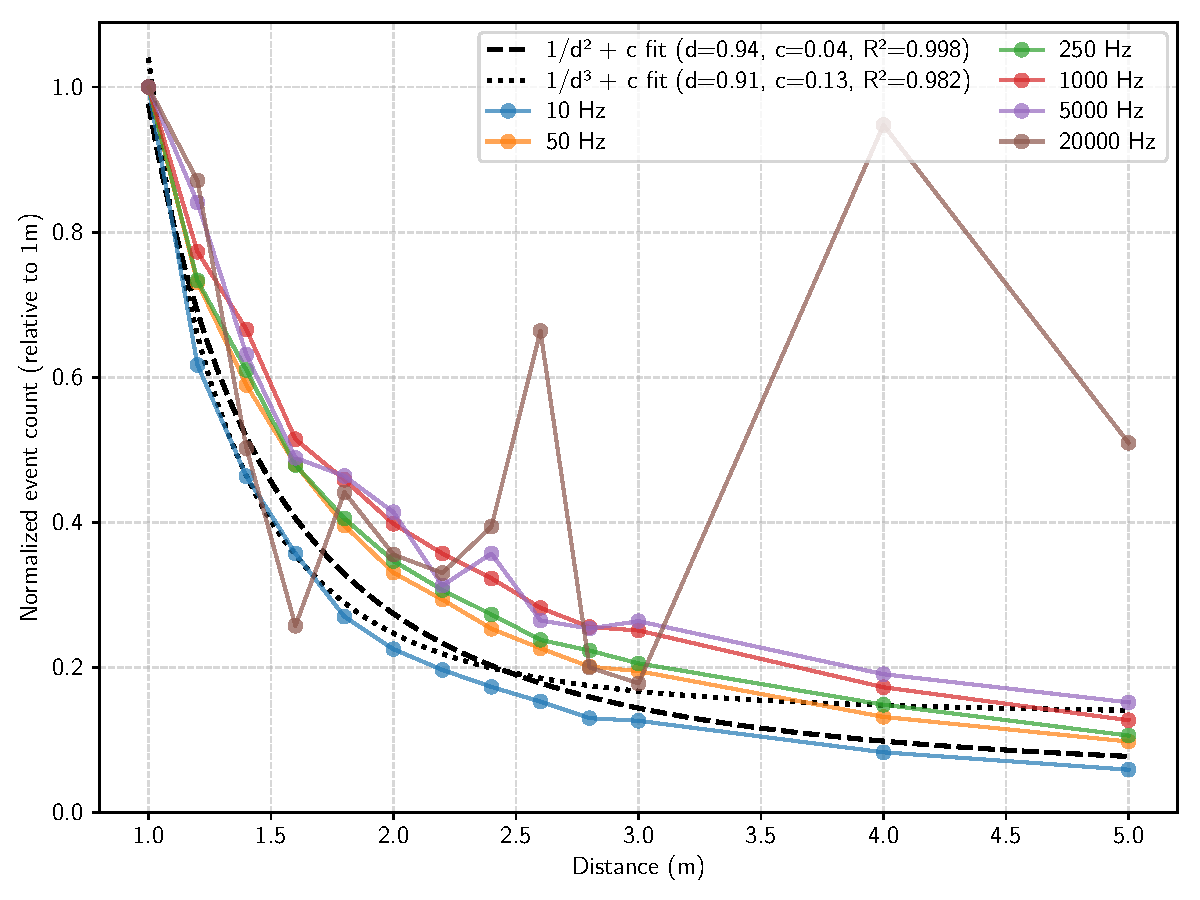
\includegraphics[width=0.70\textwidth]{../fig/pgfplot/build/inv_square.pdf}
        \label{fig:fit1}
    \end{figure}

    \vspace{-0.5cm}
    \begin{equation*}
        \text{intensity} \propto \frac{1}{\text{distance}^2}
    \end{equation*}

\end{frame}

\begin{frame}{Camera calibration}
   
   \begin{figure}[H]
        \centering
        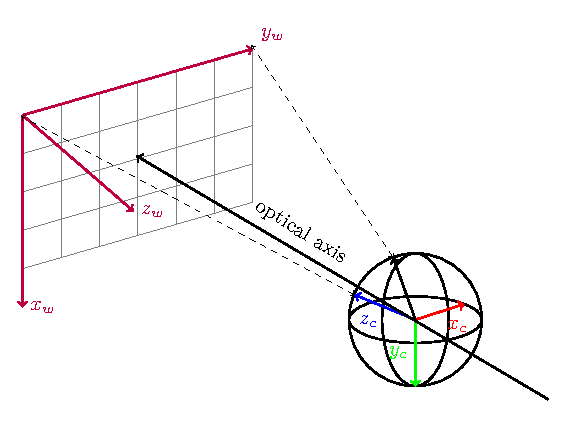
\includegraphics[width=0.8\textwidth]{../fig/tikz/extrinsic.pdf}
        %\hspace{1em}%
        %\raisebox{0.3\height}{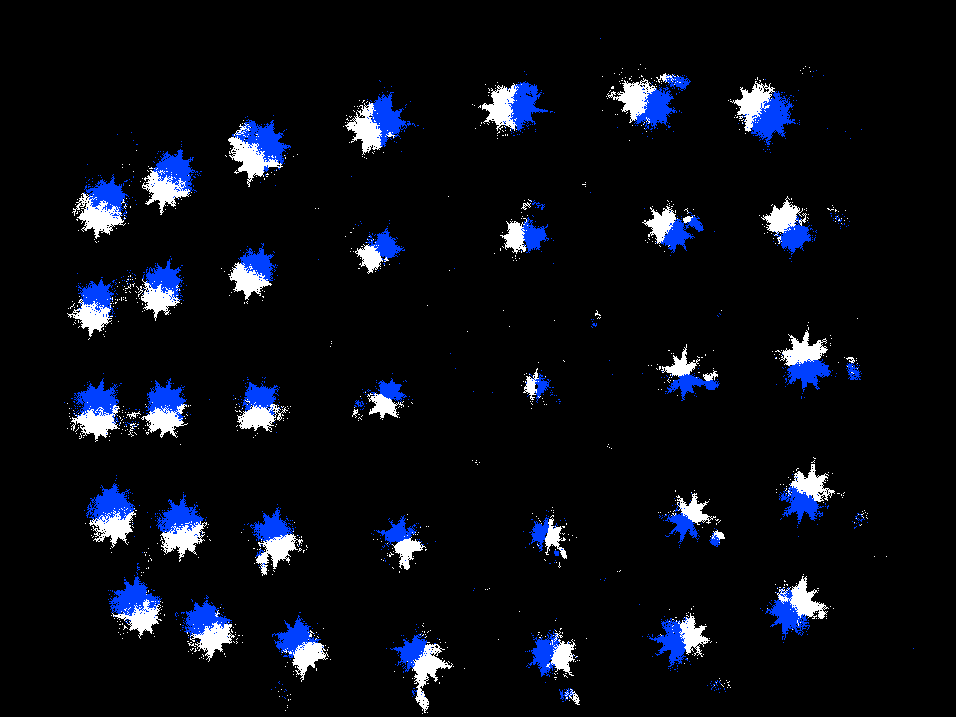
\includegraphics[width=0.3\textwidth]{../fig/photos/lattice_evs.png}}
        \label{fig:calib1}
        \caption{Camera calibration grid}
    \end{figure}
    
\end{frame}

\begin{frame}{Camera calibration}
   
   \begin{figure}[H]
	\centering
	  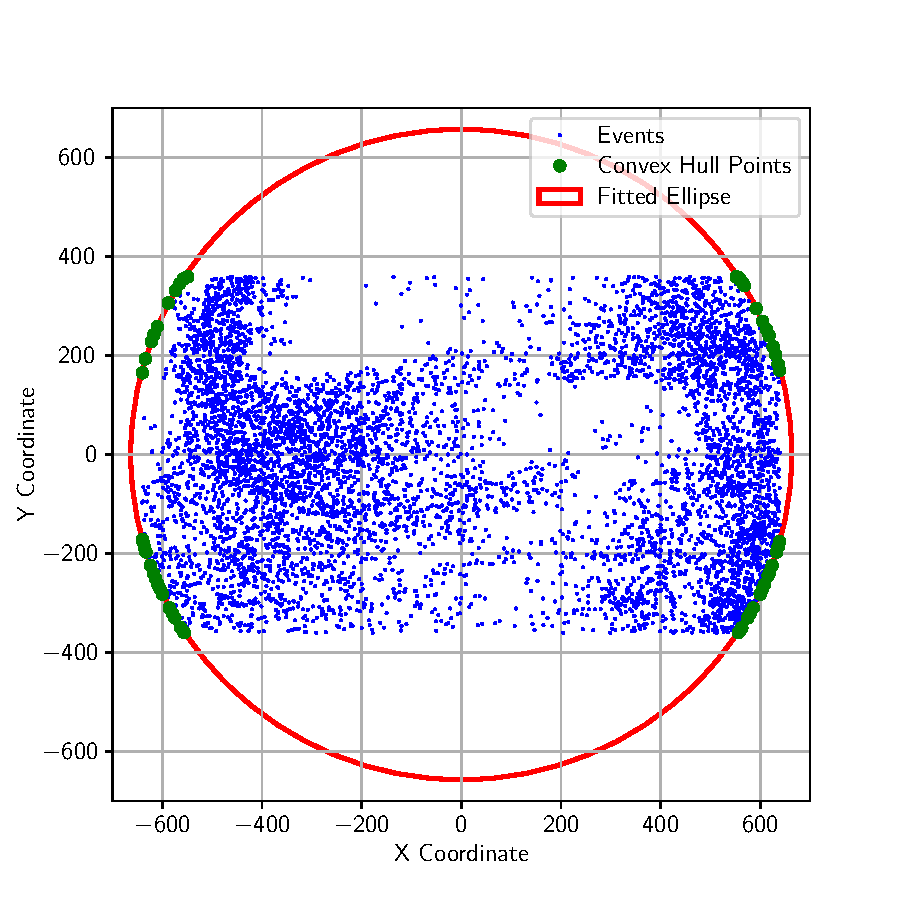
\includegraphics[width=0.35\textwidth]{./fig/pgfplot/build/ellipse_hull.pdf}
	  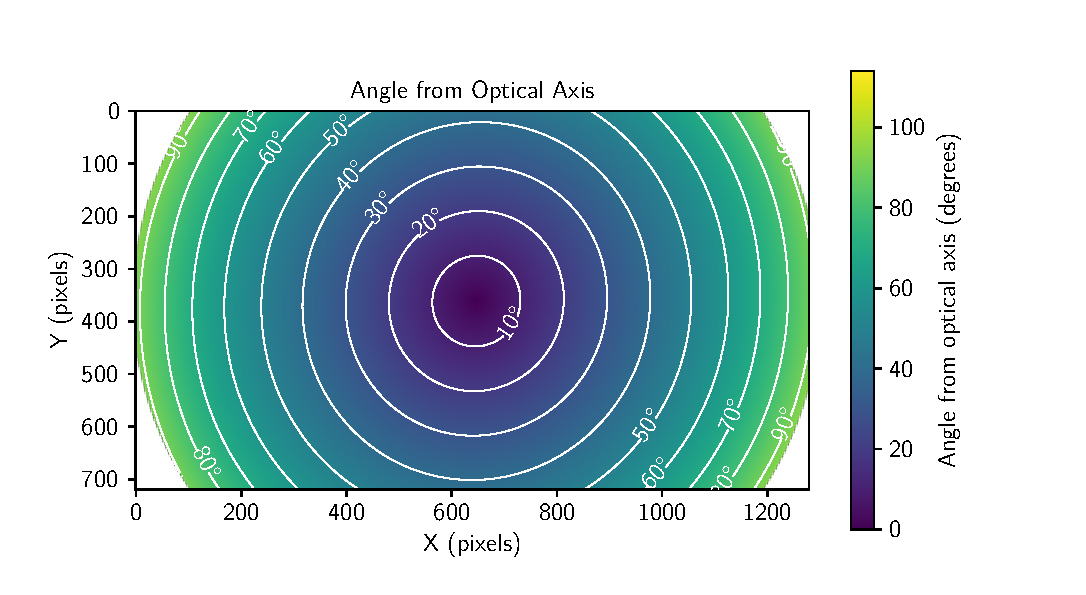
\includegraphics[width=0.6\textwidth]{./fig/pgfplot/build/evk4_viz.pdf}

	\caption{Fitting an ellipse to the visible area.}
	\label{fig:calib2}
    \end{figure}
    
\end{frame}

\begin{frame}{Calibration results}
   
   \begin{figure}[H]
	\centering
	  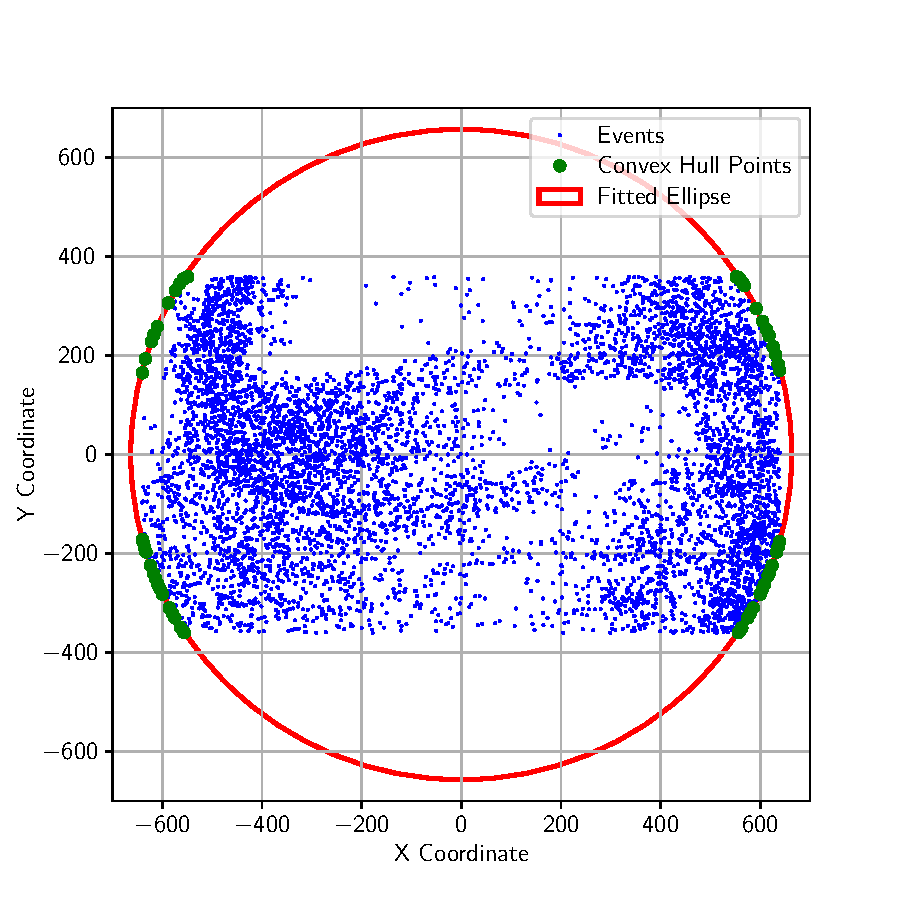
\includegraphics[width=0.35\textwidth]{./fig/pgfplot/build/ellipse_hull.pdf}
	  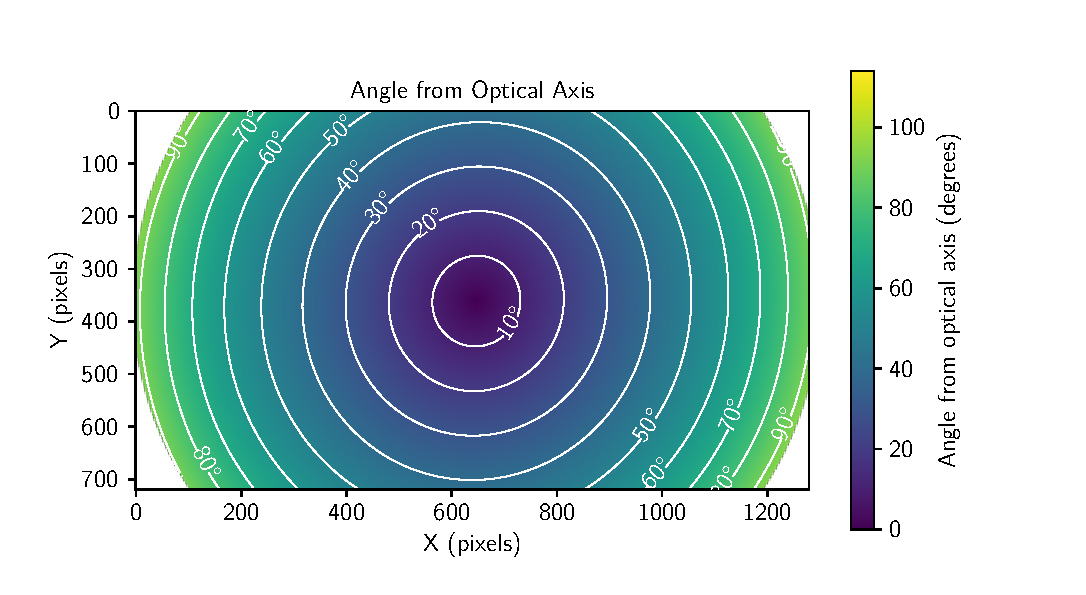
\includegraphics[width=0.6\textwidth]{./fig/pgfplot/build/evk4_viz.pdf}

	\caption{Fitting an ellipse to the visible area.}
	\label{fig:calib2}
    \end{figure}
    
\end{frame}

\begin{frame}{Perspective-n-Point}

\begin{figure}[H]
    \centering
    \raisebox{0.2\height}{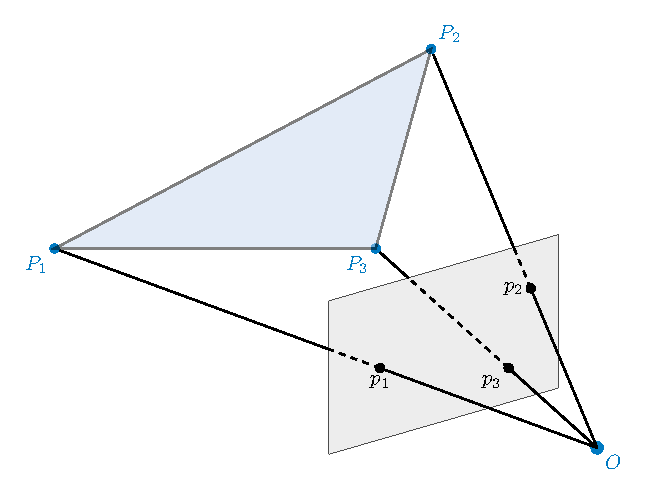
\includegraphics[width=0.55\textwidth]{../fig/tikz/p3p.pdf}}%
    \hspace{1em}%
    \raisebox{0.5\height}{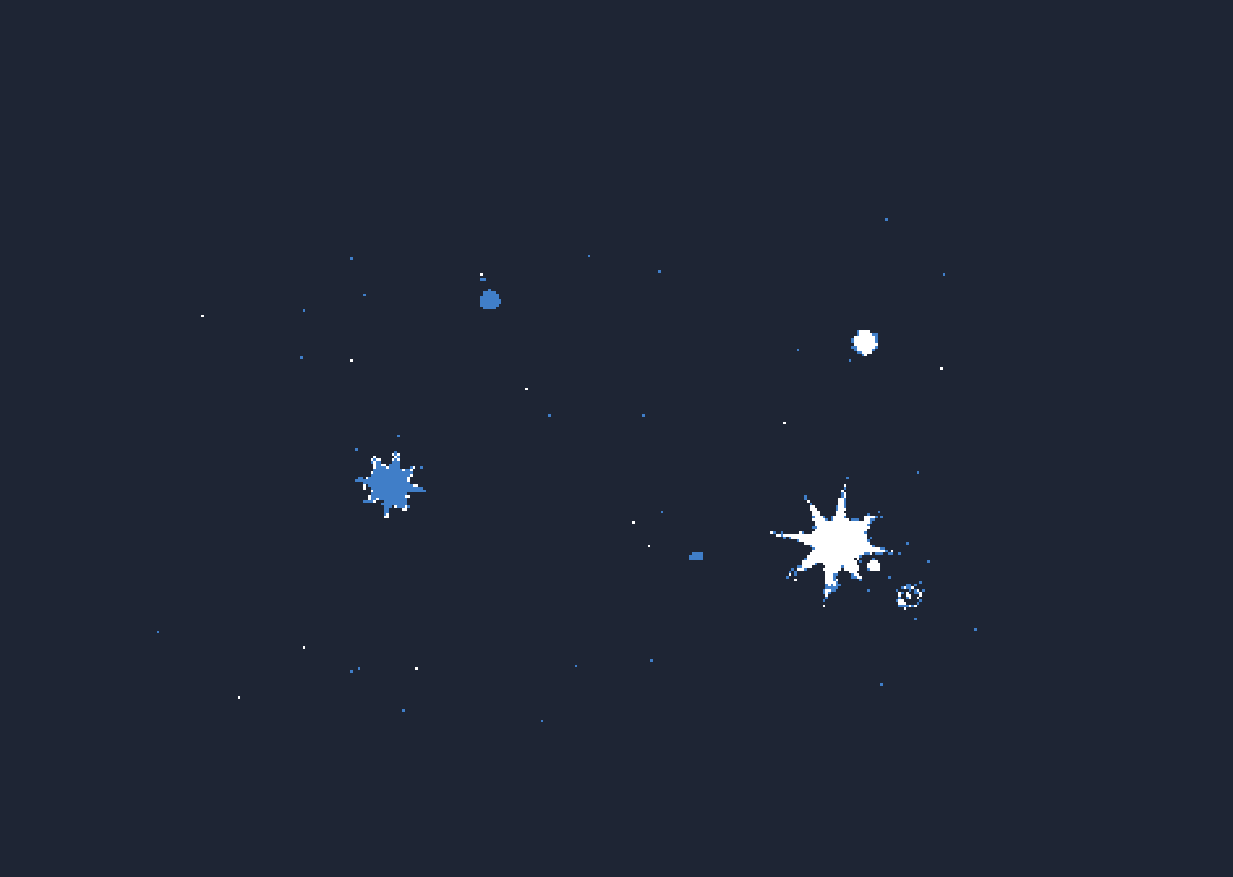
\includegraphics[width=0.40\textwidth]{../fig/photos/pnpmeas.png}}
    \label{fig:pnp}
    \caption{Perspective-n-Point visualisation.}
\end{figure}

\end{frame}

\begin{frame}{ROS implementation}

    \begin{figure}
        \centering
        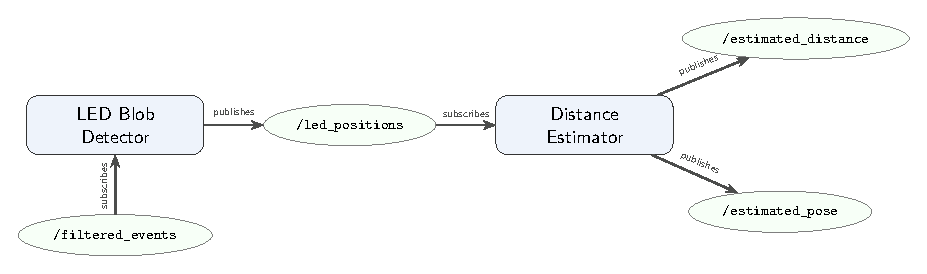
\includegraphics[width=1.0\textwidth]{../fig/tikz/rosflow.pdf}
        \label{fig:ros}
        \caption{ROS distance/position estimation pipeline.}
    \end{figure}

\end{frame}

\begin{frame}{Experiments}

\begin{figure}[H]
	\centering
	\subfloat[Static experiment] {
	  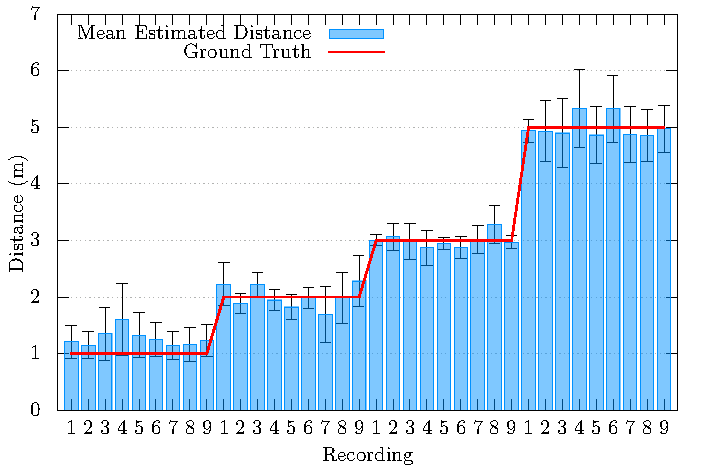
\includegraphics[width=0.45\textwidth]{../fig/tikz/pnp_results.pdf}
	  \label{fig:uav33}
	}
	\subfloat[Flying experiment] {
	  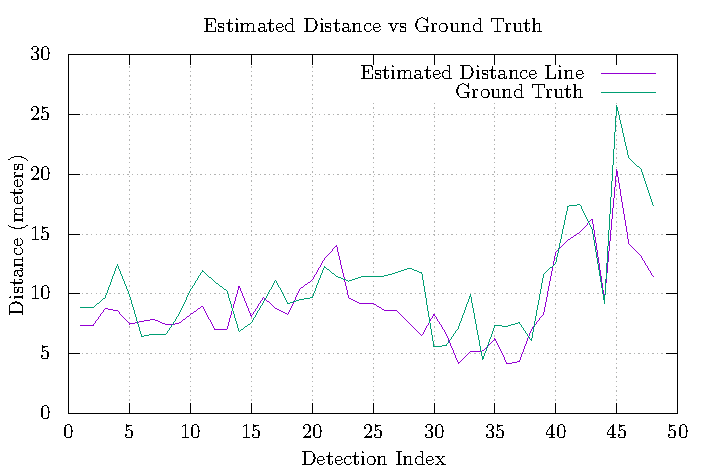
\includegraphics[width=0.49\textwidth]{../fig/tikz/experiment_analysis.pdf}
	  \label{fig:experiments}
	}
	\caption{
            The distance estimation results with a mean error of
            $0.34 \pm 0.16$ meters for the static experiment, and
            $2.47 \pm 1.75$ meters for the flying experiment.
        }
	\label{fig:uav33_37}
\end{figure}

\end{frame}

\begin{frame}{Experiments}

\begin{figure}[H]
	\centering
	  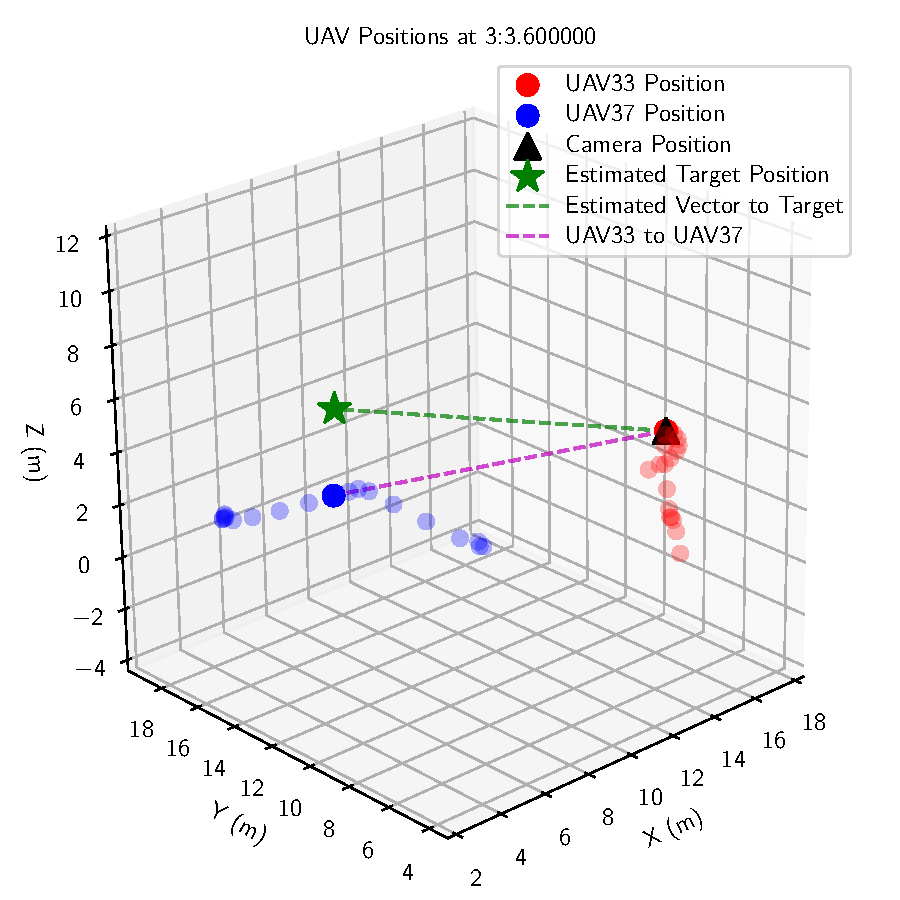
\includegraphics[width=0.45\textwidth]{../fig/pgfplot/build/3dplot3.pdf}
	  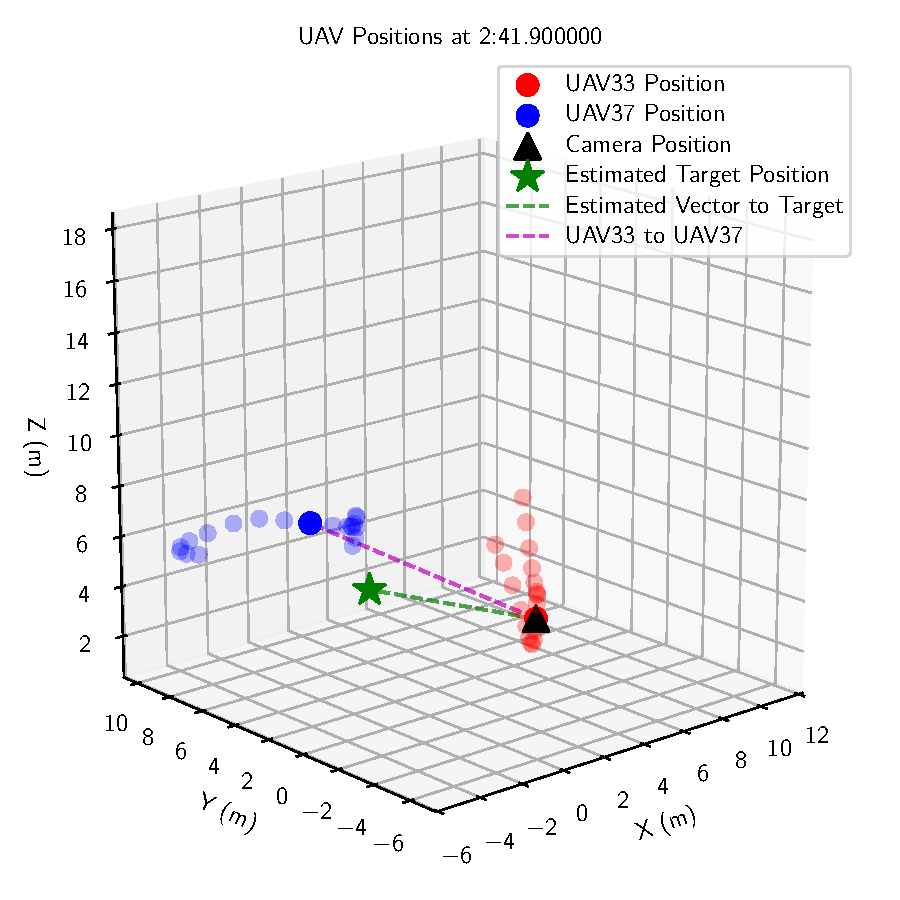
\includegraphics[width=0.45\textwidth]{../fig/pgfplot/build/3dplot1.pdf}
	\caption{
           Pose estimation results, with the estimated pose highlighted in green, and the real pose of the UAVs highlighted in red and blue.
        }
	\label{fig:poseresults}
\end{figure}

\end{frame}

% \begin{frame}[shrink=20]
%     \frametitle{References}
%     %\nocite{*}
%     \begingroup
%     \tiny
%     \printbibliography[heading=none]
%     \endgroup

%     %The source code can be found at:
    
%     %\url{https://github.com/kubakubakuba/mrs-uvdar-distance-estimator}.
% \end{frame}

\section{Questions}

\questionframe
    {Jaké jsou další metody, které by bylo možné využít k lokalizaci namísto PnP a proč bylo PnP použito namísto jich?}
    {
    \footnotesize{
    Metody pro lokalizaci založené na viditelném světle můžeme rozdělit do následujících kategorií:
        \begin{itemize}
            \item Fingerprinting - odhad polohy na základě předem naměřených referenčních vzdáleností
            \item Time/Angle of Arrival - je využit rozdíl času/úhlů doražených signálů
            \item Received Signal Strength - metoda často využívá fotodiody k poměru síly signálů
            \item Image Sensing - například PnP
        \end{itemize}
    }
    Metoda PnP bylo použita pro její možnost odhadu polohy pomocí výsledného obrázku z eventové kamery, poskytuje silný základ
    pro odhad polohy z relativně malého množství obdržených dat.
    \todo{double check, maybe rewrite}
    }

\questionframe
    {Proč se používá ”fisheye” čočka jako senzor?}
    {
    Kvůli jejímu velkému zornému poli (FOV).
    Čím větší její FOV, tím spíše jsme schopni detekovat prolétající dronu v našem zorném poli.
    }

\questionframe
    {Z jakého důvodu ve Figure 4.4 dochází k výraznému zvýšení počtu eventů pro 20kHz?}
    {
    Jedná se o šum kamery, jelikož jsou data pro každou frekvenci normalizována vzhledem k počtu eventů naměrených na jednomu metru.
    Při modulační frekvenci 20kHz byly při nastavených parametrech detekovány spíše eventy způsobené šumem,
    než reálné pixely vzniklé jako reakce na změnu jasu LED diod.
    }

\questionframe
    {Jak si vysvětlujete velkou varianci chyb při kalibraci ”fisheye” čočky? (Kapitola 4.2)}
    {
    Velká variance chyby byla nejspíše způsobena relativní nepřesností výběru středů detekovaných shluků pixelů.
    Nutno podotknout, že chyba se pohybuje pouze v řádu nižších jednotek pixelů ($\sim 1$px).
    
    \todo{? double check ?}
    }

\questionframe
    {Je průměrná chyba lokalizace (2.45 metru) vzhledem k měřeným vzdálenostem přijatelná pro praktické použití?}
    {
    Na vzdálenostech testovaných při experimentu s létajícími dronami (10 - 20 metrů) je chyba přijatelná, jelikož má samotná drona dost času reagovat na
    možné přiblížení.
    
    Námi navržený algoritmus odhaduje vzdálenost spíše nižší, než je reálná vzdálenost. Ke srážkám by tedy mělo docházet méně často.
    Na nižších vzdálenostech by chyba odhadu měla být řádově nižší, díky přesnější detekci lokace středů LED identifikátorů.
    
    \todo{? double check ?}
    }

\end{document}